\documentclass{amsart}

% For revision control
\usepackage{rcs-multi}
\rcsid{$Id$}
\rcsid{$Header$}
\rcskwsave{$Author$}
\rcskwsave{$Date$} 
\rcskwsave{$Revision$}
%%\rcsRegisterAuthor{devangel}{Dennis Jos{\'e} Evangelista}
\rcsRegisterAuthor{devangel}{Dennis J. Evangelista}

\usepackage{graphicx}
\usepackage{color}
\usepackage{siunitx}
\DeclareMathOperator*{\argmin}{\arg\!\min}
\usepackage{multirow}
\usepackage{colortbl}

% PDF metadata
\usepackage{hyperref}
\hypersetup{pdftitle={How to test for directed aerial descent?}}
\hypersetup{pdfauthor={Dennis Evangelista}}
\hypersetup{pdfsubject={biology}}
\hypersetup{pdfkeywords={biomechanics, statistics, estimation, aerodynamics, maneuverability, maximum likelihood}}


\title{How to test for directed aerial descent?}
\author{Dennis Evangelista}
\address{Department of Integrative Biology, UC Berkeley}
\email{devangel@berkeley.edu}
\thanks{Vicky Zhuang helped crystallize some of these thoughts when she and I were puzzling over how, using finite differences, some \emph{Anolis}, dropping from a ladder in Haas gymnasium, could reach accelerations of \SI[separate-uncertainty]{+-900}{\meter\per\second\squared}; Dave Bapst assured me I was not on crack.}
\date{\today}

\begin{document}
\begin{abstract}
These notes give my thoughts on how to test a recorded animal trajectory for directed aerial descent using log-likelihood functions and the Akaike Information Criterion (AIC). 
\end{abstract}
\maketitle
\tableofcontents

\section{Introduction}
In studies of the comparative biomechanics of aerial behaviors, we often obtain the trajectory of an animal traveling through space and we wish to decide if it is moving as a passive ballistic projectile would, or if it is ``doing something.'' Is it using bits of its body to generate forces and moments that change its trajectory through the air in order to right itself, land on some target, move towards some goal or away from something it wishes to avoid?  More generally, we wish to test some data and see if it is well explained by a certain model with some terms, or if an alternative model with other terms is a better description.  We may also need (or have) some idea of what our measurement noise is. 

\section{A toy example: estimating position of a stationary object with noisy measurements}
Let us imagine we have a calibrated high speed video recording of a dead limpet on a rock.  Frame by frame, we digitize the $x$ position of the limpet for the portion of the video we wish to analyze.  The data are given in Figure~\ref{fig:limpet}.  While digitizing such positions are tedious, they allow us to answer two questions.  First, what is the position of the limpet?  Second, is it still moving or is it dead?  

To answer the first question, a simple-minded thing to do first would be to simply take the mean of the measured positions.  We could report then the position as the mean along with the standard deviation; the limpet is at \SI[separate-uncertainty]{0.423+-0.001}{\meter}.  This frequentist approach is pretty standard in biology and biomechanics.  

However, we run into problems if we try to answer the second question - is the limpet still moving?  Now we must somehow approximate the derivative.  We may try using a finite difference approximation, approximating the derivative $\frac{dx}{dt}$ as $\frac{x_{n+1}-x_{n}}{\Delta t}$, then testing to see if this is significantly different from zero using an appropriately chosen frequentist statistical test.  The drawback with this is that numerical differentiation in this manner introduces noise, and since we are often after accelerations and forces, which require a second derivative, the noise can quickly mask anything interesting that may be happening in realistic data.  We could employ filters (e.g. Butterworth, Chebyshev, moving average) or interpolating spline procedures, however, these add additional layers of manipulation to the data and may be unintuitive to those not used to filtering approaches.  Furthermore, they do not make use of whatever we might happen to know about the noise in our measuring system. 

\section{An alternative using maximum likelihood estimation}
Let us proceed by imagining a model of the process of measuring the position of a dead, stationary limpet.  Unless it is being moved by something, the limpet's measured position at some discrete time $n$ may be thought of as an actual position plus some additive measurement error:
\begin{equation}
x[n] = X_0 + \mathcal{N}(0,\sigma)
\end{equation}
We might consider this model as a null model for a dead limpet.  $\mathcal{N}$ here is some model of the measurement noise; in this case for simplicity we will consider zero-mean, stationary, Gaussian noise.  For this case, it is clear that our earlier procedure of simply taking the mean and standard deviation of our measurements should recover $X_0$ as the position fo the limpet and $\sigma$ as the standard deviation, provided we take enough samples. 

Let's consider a different approach known as maximum likelihood estimation \cite{Burnham:2002, Rauch:1965}. Imagine we knew $X_0$ and $\sigma$; then we could figure out how likely it is that we observe the actual measurements by computing $P(\text{data}|\text{model},\text{parameters})$:  
\begin{equation}
\ln(\mathcal{L}(X_0,\sigma | x, \text{stationary})) = \sum_n \ln \left(f_{\mathcal{N}(0,\sigma)}(x[n]-X_0) \right)
\end{equation}
$\ln(\mathcal{L})$ is the log-likelihood; it is easier for us to use because it turns the product of many small numbers into a sum of something that is more easily represented within the computational range of our computer.  To figure out the most likely estimate of the position of the limpet (and the noise of our measuring setup), we can search for the values of those parameters that maximize the likelihood:
\begin{equation}
\hat{X_0}, \hat\sigma = \argmin_{X_0, \sigma} \left[ - \sum_n \ln \left(f_{\mathcal{N}(0,\sigma)}(x[n]-X_0) \right) \right]
\label{eq:MLE}
\end{equation}
The search is done in our computer, using whatever minimum-seeking routine we wish to use, such as various flavors of \texttt{fmin} in Matlab, Octave or Python, ``GoalSeek'' in ExcelSucks, etc.  

At first glance, the log-likelihood approach appears to make life more complicated, but it is an improvement.  With our old approach, we heavily manipulate the data to get velocities and accelerations, compute some test statistics (mean, standard deviation) and then perform some set, voodoo-like procedure (ANOVA or non-parametric test) to see if this is different from the position of another dead limpet.  The test procedure is, to many biomechanics practitioners, a black box relegated to a stats course taken long ago.  The old approach is ``no thought required'' - which is precisely its drawback.  By instead modeling the process that produced the measurements, we can get a handle on both the physical process driving the measurement and the measurement noise.  We can also then compare different models, to select which is a more appropriate description of what we have observed.

\section{Comparing models}
Back to the question of is the limpet moving?  Our null approximating model (repeated below) was that it is stationary: 
\begin{equation}
g_0:  x[n] = X_0 + \mathcal{N}(0,\sigma)
\label{eq:stationary}
\end{equation}

A reasonable alternative approximating model is that the limpet is crawling along with some constant velocity $V$:
\begin{equation}
g_1:  x_v[n] = X_0 + V \frac{n}{f} + \mathcal{N}(0,\sigma)
\label{eq:constantv}
\end{equation}
where the positions are sampled at some known sample rate $f$; this is simply $x=X_0+Vt$.  We could perform a log-likelihood calculation for $g_1$ and get a decent guess for what $X_0$, $V$ and $\sigma$ are for that model, noting that we've added an additional parameter $V$.  We might like to know if the data are better explained by $g_0$ or $g_1$? Additionally, if $g_1$ is ``better'', is it better by enough to justify the additional parameter $V$, or are we guilty of what is known as \emph{over fitting}?

\subsection{Akaike information criterion (AIC)}
The Akaike information criterion (AIC) \cite{Akaike:1974} provides a way to compare several candidate approximating models and ask if the additional explanatory power of a given model is worth the extra parameters ($k$ is the number of parameters):  
\begin{equation}
\mbox{AIC} = 2 k - 2 \ln(\mathcal{L})
\end{equation}
The AIC is computed for the maximum likelihood parameter estimate for each model.  The model that best explains the data is the one with the minimum AIC value.  In essence, we are searching for the model that requires as little information as necessary to describe the observed data well.  

We can see that increasing the number of parameters increases the AIC. On the other hand, a model that is more likely to explain the observed data will have a smaller AIC.  Models within 1-2 of the minimum have substantial support and should not be discarded; models within 4-7 have less support and models 10 and above have no support and can be discarded \cite{Akaike:1974, Burnham:2002}.  

%There are alternatives to this procedure; a likelihood ratio test could be used, or an equivalent Bayesian approach adopted.  I am not able enough in probability and statistics to make sense of these yet and the AIC appears to fit my needs.  

%PARAPHRASE- Akaike weights are can be used in model averaging. They represent the relative likelihood of a model. To calculate them, for each model first calculate the relative likelihood of the model, which is just exp( -0.5 * �AIC score for that model). The Akaike weight for a model is this value divided by the sum of these values across all models.
%
%DAVE BAPST NOTES - I'd use AIC weights rather than change in AIC. AIC weights are more easily interpretable for assessing model support. Check Burnham and Anderson for the equation. Gene Hunt has a nice akaike.wts() function in R in his paleoTS library. I'm pretty certain you can do the same thing with the BIC.
%
%DAVE BAPST NOTES - Likelihood ratio tests can only be used if two models are nested, which I think may be the case here (does setting V=0 collapse one model into the other? I think it does.) They are considered 'better' than AIC or BIC (by some people), but you can only compare pairs of models with them and they must be nested. Bayesian analyses are nice in some ways, but its unclear to me why you would want to go that route here. The likelihood method is just simpler and more understandable to non-statistically minded people. If you aren't going to use LRT or Bayesian analysis, I would just drop any mention of those methods.

\subsection{Bayesian information criterion (BIC)}
An alternative to AIC is the Bayesian information criterion (BIC) \cite{Schwarz:1978}.  It is similar in form but includes a term related to the number of observations $n$.  This means that the penalty for having more parameters is larger than in the AIC.  We can check both and see if similar answers are given with each index.
\begin{equation}
\mbox{BIC} = k \ln(n) - 2 \ln(\mathcal{L}) 
\end{equation}



\subsection{So is the limpet moving?}
Let us apply these to some (simulated) limpet data for two limpets, shown in Figure~\ref{fig:limpet}:
\begin{figure}
\includegraphics[width=\textwidth]{figures/Limpet2.jpg}
\caption{Simulated limpet data. Limpet 1 is blue, Limpet 2 is green.}
\label{fig:limpet}
\end{figure}
The simple estimate of the position of Limpet 1 is \SI[separate-uncertainty]{0.423+-0.001}{\meter}, obtained by taking the mean and standard deviation.  If we apply the maximum likelihood estimation algorithm of Equation~\ref{eq:MLE} to Limpet 1, we obtain the same, \SI[separate-uncertainty]{0.423+-0.001}{\meter}.  It's nice to get the right answer (these correspond to the ``true'' values for Limpet 1 in the simulation), and we can go a little further.

We wish to test if the limpets are moving, by checking which fits the data best, stationary model $g_0$, or constant velocity model $g_1$.  Tables~\ref{tbl:limpet} and \ref{tbl:limpet2} summarize the maximum likelihood estimates for the limpets for each model.  The table also contains the AIC and BIC values for the models.  Limpet 1 is stationary and the model with a constant velocity term estimates zero speed (Table~\ref{tbl:limpet}).  We conclude that Limpet 1 is not moving.  On the other hand, there is substantial support that Limpet 2 is moving to the right (Table~\ref{tbl:limpet2}, $\Delta_i\;\text{AIC} = \num{61.1}$).  Comparing the $\Delta_i\;\text{AIC}$ and $\Delta_i\;\text{BIC}$ shows that the constant velocity model has substantially more explanatory power for Limpet 2.  Limpet 2 is not dead, it is moving to the right at \SI{0.0001}{\meter\per\second} (which is also the ``true'' value for Limpet 2 in the simulation). 
 
Note that taking finite differences of the data in Figure~\ref{fig:limpet} would have been hopelessly fracked by the measurement noise; the mean speed of Limpet 2 by that method is \SI{-8.9e-5}{\meter\per\second}.  The ``true'' values here would have been very hard to pick out of the noisy data using simple finite differences.

%\begin{table}
%\begin{tabular}{lrrrr}
% & \multicolumn{2}{c}{Limpet 1} & \multicolumn{2}{c}{Limpet 2} \\
%%         & Limpet 1 & Limpet 1 & Limpet 2 & Limpet 2\\
%         & \textbf{stationary} & constant v & stationary & \textbf{constant v}\\
%$\sigma$, \SI{}{\meter} & \num{0.001} & \num{0.001} & \num{0.0012} & \num{0.0009}\\
%$X_0$, \SI{}{\meter}    & \num{0.423} & \num{0.423} & \num{0.4235} & \num{0.423}\\
%$V$, \SI{}{\meter\per\second}  & \num{} & \num{0.000} & \num{} & \num{0.0001} \\ 
%\vspace{1ex}\\
%$\ln(L)$ & \num{3308.2} & \num{3308.2} & \num{3308.8} & \num{3340.3} \\
%AIC & \num{-6612.3} & \num{-6610.3} & \num{-6613.5} & \num{-6674.6} \\
%$\Delta\mbox{AIC}$ & \num{} & \num{2.0} & \num{61.1} & \num{} \\
%BIC & \num{-6603.5} & \num{-6597.1} & \num{-6604.7} & \num{-6667.8} \\
%$\Delta\mbox{BIC}$ & \num{} & \num{6.4} & \num{63.1} & \num{} \\
%\end{tabular}
%\end{table}

\begin{table}
\caption{Maximum likelihood parameter estimates and model comparison information for Limpet 1 in the simulated data of Figure~\ref{fig:limpet}.  The generating model (``truth'') for Limpet 1 is stationary at $X_0 = \SI{0.423}{\meter}$.} 
\label{tbl:limpet}
\begin{tabular}{lccccccccc}
      & \multicolumn{3}{c}{Parameter estimates} & \multicolumn{6}{c}{Model comparison information} \\
Model & $\sigma$, \SI{}{\meter} & $X_0$, \SI{}{\meter} & $V$, \SI{}{\meter\per\second} & $K$ & $MSE$ & $\ln{(\mathcal{L})}$ & $\Delta_i\;\text{AIC}$ & $\Delta_i\;\text{BIC}$ & $w_i$ \\
\hline 
\rowcolor[gray]{0.8} $g_0$, stationary & \num{0.001} & \num{0.423} & \num{} & 2 & & \num{3308.2} & \num{0.0} & \num{0.0} & \\
$g_1$, constant v & \num{0.001} & \num{0.423} & \num{0.000} & 3 & & \num{3308.2} & \num{2.0}& \num{6.4} & \\
%$g_2$, constant a & & & & 4 & & & & & \\
\end{tabular}
\end{table}

\begin{table}
\caption{Maximum likelihood parameter estimates and model comparison information for Limpet 2 in the simulated data of Figure~\ref{fig:limpet}. The generating model for Limpet 2 is moving right at $V=\SI{0.0001}{\meter\per\second}$.} 
\label{tbl:limpet2}
\begin{tabular}{lccccccccc}
      & \multicolumn{3}{c}{Parameter estimates} & \multicolumn{6}{c}{Model comparison information} \\
Model & $\sigma$, \SI{}{\meter} & $X_0$, \SI{}{\meter} & $V$, \SI{}{\meter\per\second} & $k$ & $MSE$ & $\ln{(\mathcal{L})}$ & $\Delta_i\;\text{AIC}$ & $\Delta_i\;\text{BIC}$ & $w_i$ \\
\hline
$g_0$, stationary & \num{0.0012} & \num{0.4235} & \num{} & 2 & & \num{3308.8} & \num{61.1} & \num{63.1} & \\
\rowcolor[gray]{0.8} $g_1$, constant v & \num{0.0009} & \num{0.423} & \num{0.0001} & 3 & & \num{3340.3} & \num{0.0}& \num{0.0} & \\
%$g_2$, constant a & & & & 4 & & & & & \\
\end{tabular}
\end{table}


\section{Real example:  Angry Bird / Ping pong ball}

Rather than just testing with simulated data, we wish to check our methods with a real, physical example of a passive projectile in flight.  This will allow us to check the performance of our techniques given realistic noise from typical biomechanics data gathering setups.  

We filmed the trajectory of a commercially available toy (Angry Birds\footnote{The physical toy was inspired by a popular computer game in which various birds are shot by a slingshot at structures containing evil green pigs.  Analysis of the game physics used shows that either the birds are \SI{5}{\meter} tall \cite{Allain:2010}, heights only seen in extinct, non-volant birds; or the computer game does \emph{not} conform to our normal rules of physics; for example $g$ is substantially less than \SI{9.8}{\meter\per\second\squared}.  } Knock on Wood Game, Mattel Inc., El Segundo, CA) consisting of a spring-powered catapult and (approximately) spherical, 1-inch (\SI{2.54}{\centi\meter}) projectile, mass \SI{5.88}{\gram}.  The trajectory was filmed at \SI{60}{frame\per\second} using a fixed-focus HD camcorder (Flip MinoHD; Cisco Systems, San Jose, CA) placed perpendicular to the plane of movement.  Calibration was provided by a \SI{15}{\centi\meter} scale placed in view of the camera.  Projectile positions were digitized on a MacBook Pro (Apple; Cupertino, CA) using a freely available software package (GraphClick; Arizona Software).  Subsequent analysis, described in detail below, was carried out in R \cite{R:2011}.    

A typical trajectory is given in Figure~\ref{fig:redbird1}. The digitized result is shown in Figure~\ref{fig:redbird2}. 

\begin{figure}
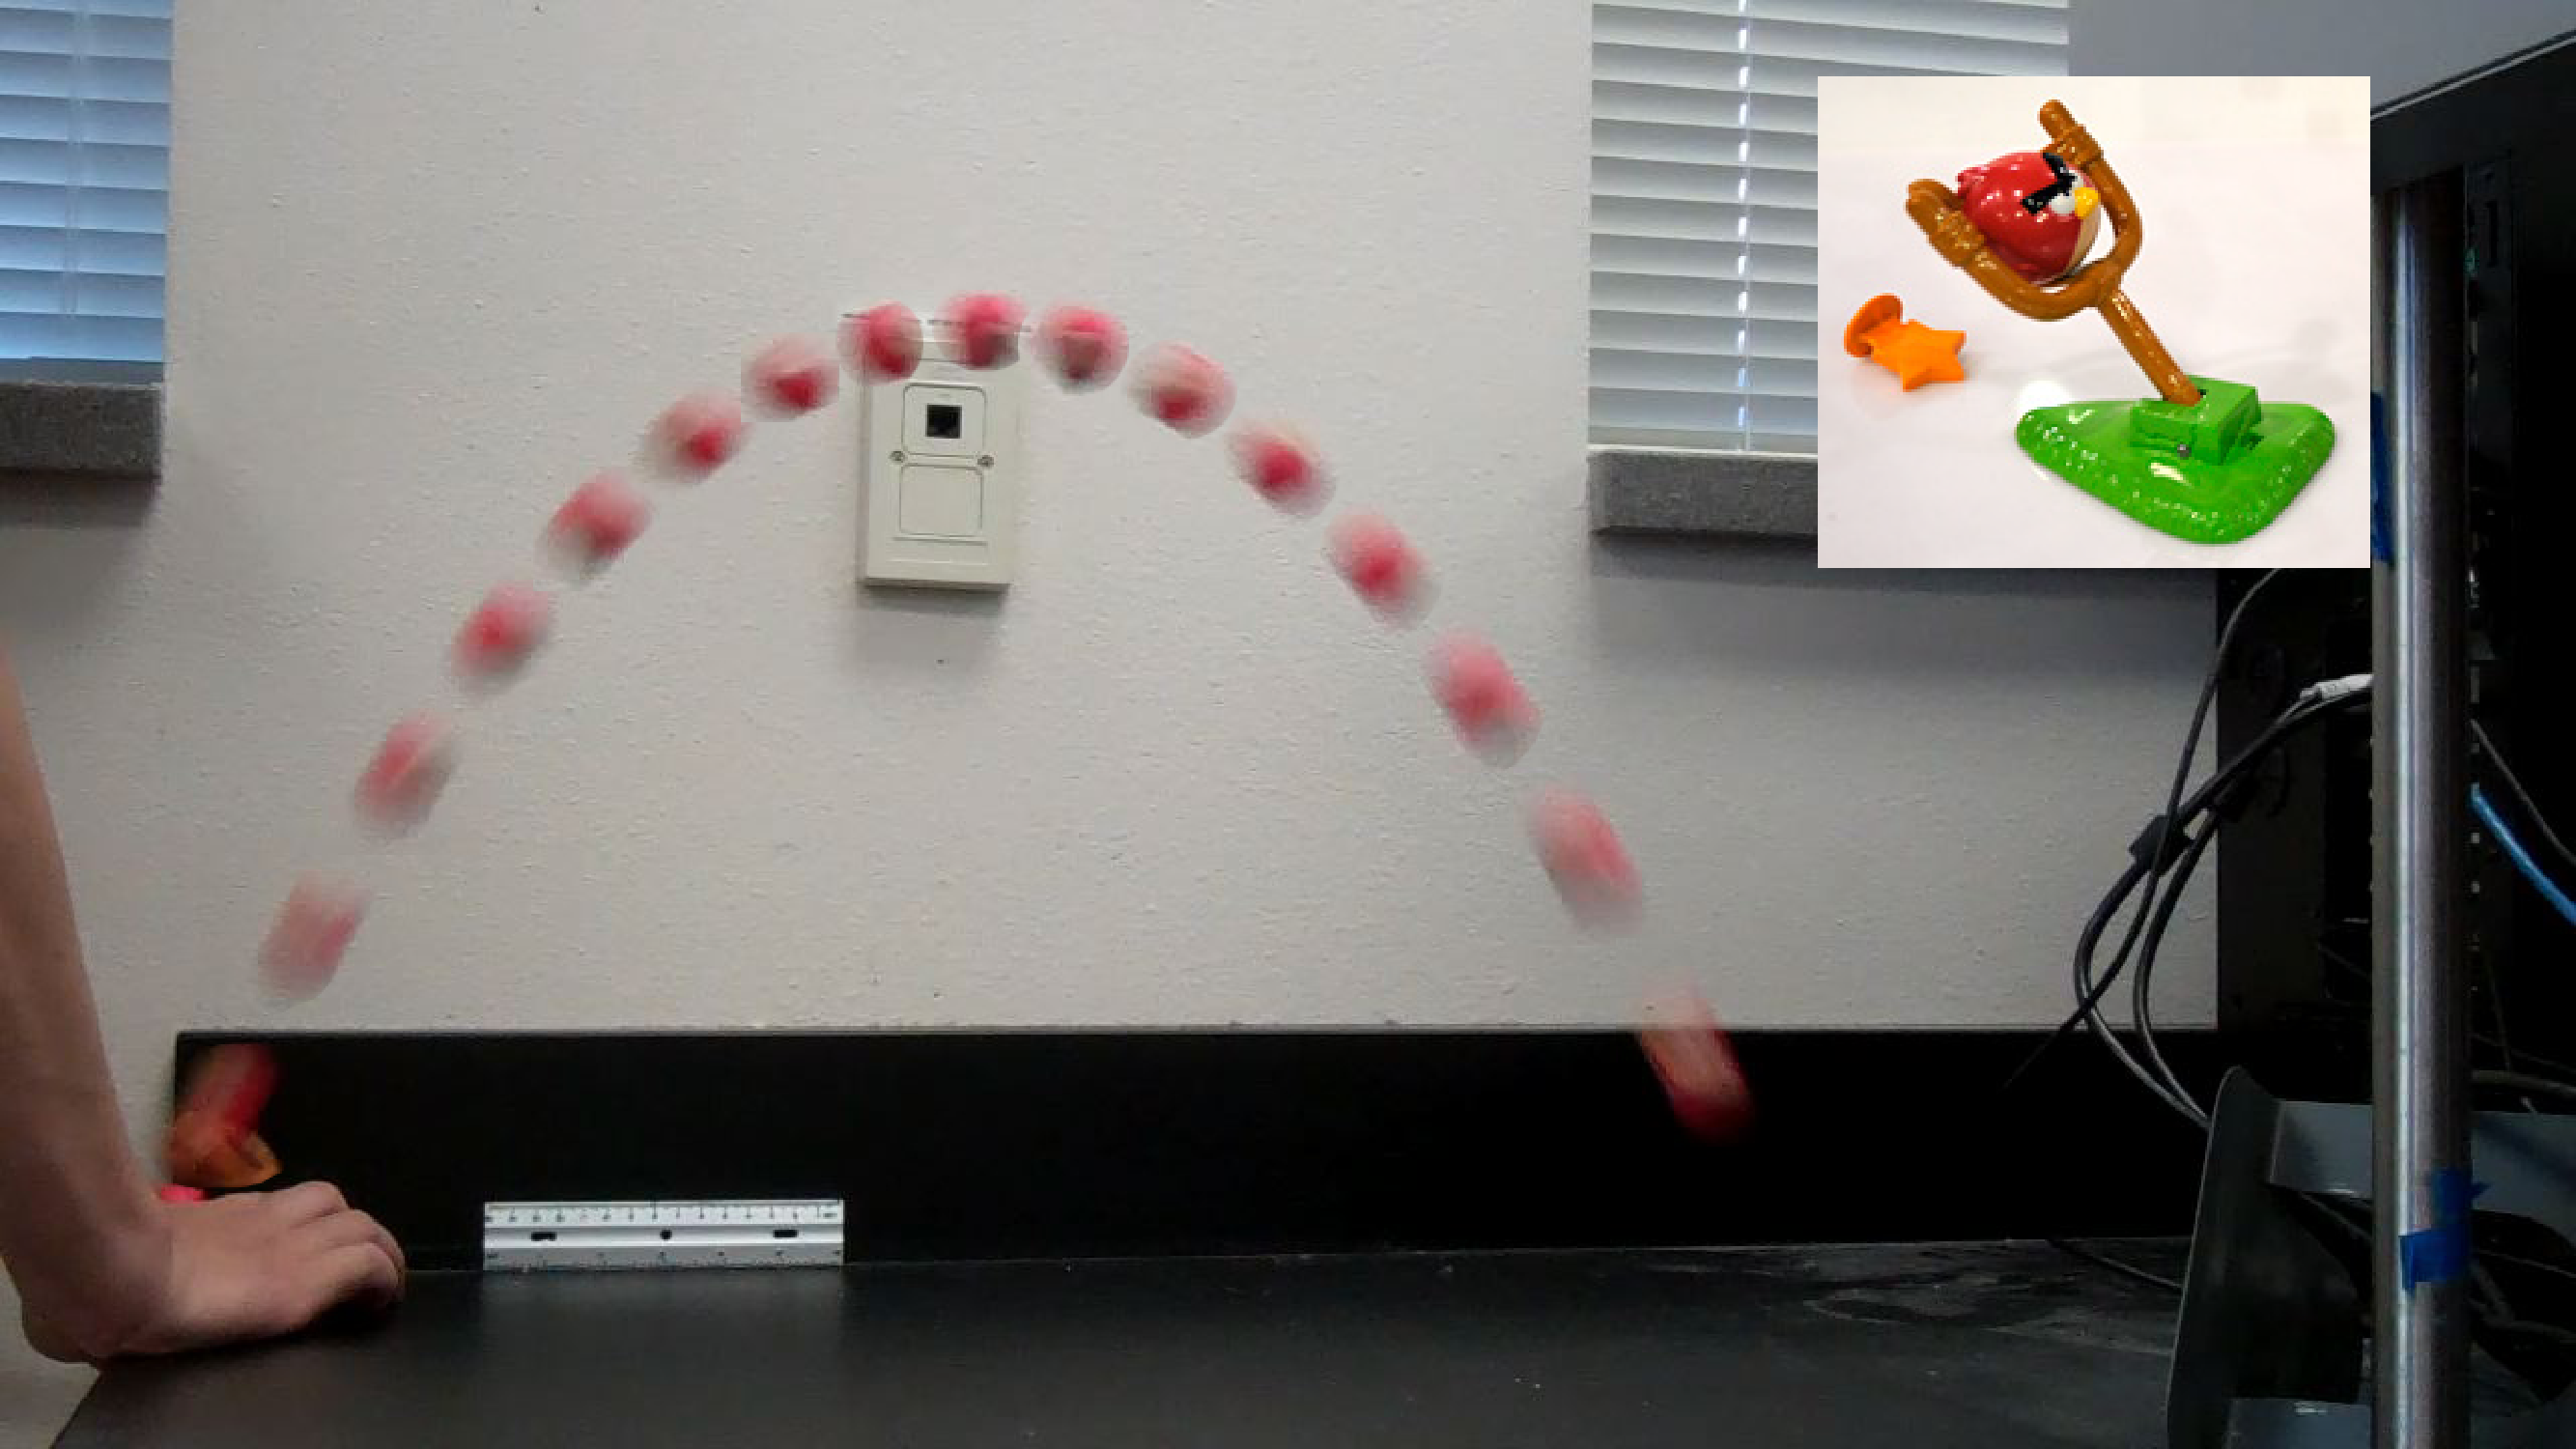
\includegraphics[width=\textwidth]{figures/angry-bird-trajectory/AngryBirdComposite.pdf}
\caption{Trajectory of an Angry Bird.  Composite image with multiple frames superimposed, \SI{30}{frame\per\second}, elapsed time approximately \SI{0.5}{\second}. Scale \SI{15}{\centi\meter}.  Inset shows catapult device and projectile.}
\label{fig:redbird1}
\end{figure}

\begin{figure}
\includegraphics[width=\textwidth]{figures/angry-bird-mle/angrybird2.pdf}
\caption{Digitized trajectory of an Angry Bird.  Body positions at \SI{1/60}{\second} intervals shown by dots. Blue line shows the best supported candidate models for $x(t)$ and $y(t)$.  Red line shows an unsupported candidate model.  It would be nice to add some kind of confidence interval or bootstrapping indication.}
\label{fig:redbird2}
\end{figure}

To continue with the analysis, we construct several physically-motivated candidate approximating models that we will then test to see which is best supported by the data:  

\begin{align}
\notag g_0:  x &= X_0 + \mathcal{N}(0,\sigma)& &\text{(stationary)}\\
\notag g_1:  x &= X_0 + V t + \mathcal{N}(0,\sigma)& &\text{(constant velocity)}\\
\notag g_2:  x &= X_0 + V t + \frac{1}{2}a t^2 + \mathcal{N}(0,\sigma)& &\text{(constant acceleration)}\\
\notag g_2':  x &= X_0 + V t - \frac{1}{2} \num{9.81} t^2 + \mathcal{N}(0,\sigma)& &\text{(Earth gravity)}\\
%\notag g_3:  x &= X_0 + V t + \frac{1}{2}a t^2 +\frac{1}{6}b t^3 + \mathcal{N}(0,\sigma)& &\text{(constant jerk)}\\
\notag g_3:  x &= X_0 + V t + X_1 e^{-t/\tau} + \mathcal{N}(0,\sigma)& &\text{(linear drag terminal velocity)}
\end{align}

For simplicity we consider similar forms for $y$ and assume that noise in $x$ and $y$ are uncorrelated, stationary, zero-mean Gaussian random processes $\mathcal{N}(0,\sigma)$.  Also, for a more complicated example, we might construct and solve a system of differential equations describing the motion \cite{Rauch:1965} (or see the next section). Here we work only with the trivial known forms of the solutions for simple cases. These should be adequate to describe the motion, but if they are not, we will find out from a poor fit and a large noise variance $\sigma$. 

The models were then used along with the \texttt{mle2} routine in R to obtain maximum likelihood estimates and values for the log-likelihood, AIC and BIC.  The results of the analysis are given in Tables~\ref{tbl:redbirdx} and \ref{tbl:redbirdy}. The best supported models are constant velocity ($g_1$) in $x$ and Earth gravity ($g_2'$) in $y$.  These are shown as the blue line in Figure~\ref{fig:redbird2}.  In contrast, an unsupported model, such as constant velocity ($g_1$) in $y$, shown as the red line in Figure~\ref{fig:redbird2} gives a poor fit as well as large $\Delta_i$ AIC and BIC values and low likelihood values (comparable to stationary in Table~\ref{tbl:redbirdy}).

AIC weights?

Say something about terminal velocity?  And other candidate models? mle2 seems not to be the best at finding minima without crashing into badness but we can fix that by tweaking the initial guess. Also the placement of tables 3 and 4 is somewhat problematic because of where latex wants to put the floats.  Sigh.

Compare to if we blindly took two finite differences of the raw data. Blah blah blah.   

Say something about how this can then be used to see if something is doing something other than what a passive projectile would do.  If the Angry Bird had a magic thruster that it was using to steer around a girder and come at an evil green pig from behind, we should see that by seeing that the models for passive projectiles are not supported by the altered trajectory.  

\begin{table}
\caption{Maximum likelihood parameter estimates and model comparison information for Angry Bird trajectory $x$ data of Figure~\ref{fig:redbird2}.} 
\label{tbl:redbirdx}
\begin{tabular}{lSSSSSS}
$x$ model & {$\sigma$, \SI{}{\meter}} & {$X_0$, \SI{}{\meter}} & {$V$, \SI{}{\meter\per\second}} & {$a$, \SI{}{\meter\per\second\squared}} & {$X_1$, \SI{}{\meter}} & {$\tau$, \SI{}{\second}} \\
\hline
$g_0$, stationary & \num{0.210} & \num{0.331} & \num{} & \num{} & \num{} & \num{} \\
\rowcolor[gray]{0.8} $g_1$, constant v & \num{0.007} & \num{-0.023} & \num{1.248} & & & \\
$g_2$, constant a & \num{0.005} & \num{-0.013} & \num{1.144} & \num{0.365} & & \\
$g_2'$, Earth gravity & \num{0.129} & \num{-0.279} & \num{4.031} & \num{-9.810} & & \\
$g_3$, terminal v & \num{0.010} & \num{-0.708} & \num{1.660} & \num{} & \num{0.693} & \num{1.374} \\
\end{tabular}

\begin{tabular}{lcccc}
$x$ model & $k$ & $\ln(\mathcal{L})$ & $\Delta_i\;\text{AIC}$ & $\Delta_i\;\text{BIC}$ \\
\hline
$g_0$, stationary & 2 & \num{4.93} & \num{260.2} & \num{257.1}  \\
\rowcolor[gray]{0.8} $g_1$, constant v & 3 & \num{137.03} & \num{0.0} & \num{0.0} \\
$g_2$, constant a & 4 & \num{125.75} & \num{20.6} & \num{19.0} \\
$g_2'$, Earth gravity & 3 & \num{21.98} & \num{228.1} &  \num{226.5} \\
$g_3$, terminal v & 4 & \num{-32.16} & \num{340.4} & \num{341.9} \\
\end{tabular}
\end{table}

\begin{table}
\caption{Maximum likelihood parameter estimates and model comparison information for Angry Bird trajectory $y$ data of Figure~\ref{fig:redbird2}.} 
\label{tbl:redbirdy}
\begin{tabular}{lcccccc}
$y$ model & $\sigma$, \SI{}{\meter} & $X_0$, \SI{}{\meter} & $V$, \SI{}{\meter\per\second} & $a$, \SI{}{\meter\per\second\squared} & $X_1$, \SI{}{\meter} & $\tau$, \SI{}{\second} \\
\hline
$g_0$, stationary & \num{0.126} & \num{0.238} & \num{} & \num{} & \num{} & \num{} \\
$g_1$, constant v & \num{0.127} & \num{0.224} & \num{0.052} & & & \\
$g_2$, constant a & \num{0.010} & \num{-0.036} & \num{2.877} & \num{-9.955} & & \\
\rowcolor[gray]{0.8} $g_2'$, Earth gravity & \num{0.010} & \num{-0.032} & \num{2.835} & \num{-9.810} & & \\
$g_3$, terminal v & \num{0.010} & \num{3.882} & \num{-4.647} & \num{} & \num{-3.937} & \num{0.484} \\
\end{tabular}

\begin{tabular}{lcccc}
$y$ model & $k$ & $\ln(\mathcal{L})$ & $\Delta_i\;\text{AIC}$ & $\Delta_i\;\text{BIC}$ \\
\hline
$g_0$, stationary & 2 & \num{22.56} & \num{175.4} & \num{173.9}  \\
$g_1$, constant v & 3 & \num{22.65} & \num{177.3} & \num{177.3} \\
$g_2$, constant a & 4 & \num{111.87} & \num{0.8} & \num{2.4} \\
\rowcolor[gray]{0.8} $g_2'$, Earth gravity & 3 & \num{111.28} & \num{0.0} &  \num{0.0} \\
$g_3$, terminal v & 4 & \num{-32.17} & \num{290.9} & \num{294.0} \\
\end{tabular}
\end{table}



\section{Real example:  Paper airplane}

%\section{Real example:  Amphipod, Lizard, Chukar falling}
\section{Conclusions}
It is possible to test for aerial behaviors with a minimum of statistical voodoo.  There is still some voodoo, but it is confined to a few, easy-to-understand places and one can at least rationalize the form the voodoo takes. We will now go apply what we have learned to a number of actual biological systems - amphipods, falling chukar, etc.  I might also try to use these methods on the phased array problem, and on the falling animal death curve.

% AMS style references
\bibliographystyle{amsplain}
\bibliography{references/tdd}
\end{document}
